\documentclass[../report/report.tex]{subfiles}
%\usepackage{algpseudocode}
\begin{document}
So far we have considered general graphical model where pair-wise connections might be defined between all the nodes. However, we are interested in the adaptation of the EMF to the restricted Boltzmann machine.
\subsection{Adaptation of TAP to RBM}
To obtain the division between visible and hidden layers lets define visible and hidden magnetizations denoted by $\mathbf{m}^\mathbf{v}$ and $\mathbf{m}^\mathbf{h}$ respectively. The energy in the BM model is set to $1$ thus we set $\beta$ to $1$ as well. This leads to the following free energy expansion (up to the third term) in the new setting:
\begin{align}
\begin{split}
G(\mathbf{m^v},\mathbf{m^h}) ~\simeq & ~H(\mathbf{m^v}, \mathbf{m^h}) \\
&  - \sum_i a_i m_i^v - \sum_j b_j m_j^h \\
 & - \sum_{i,j} \left( 
 m_i^v w_{ij} m_j^h +  \frac{w_{ij}^2}{2}(m_i^v - (m_i^v)^2)(m_j^h - (m_j^h)^2) 
  \right) \\
    &  - \sum_{i,j} \left( 
 \frac{2w_{ij}^3}{3}(m_i^v - (m_i^v)^2)(\frac{1}{2} - m_i^v)(m_j^h - (m_j^h)^2)(\frac{1}{2} - m_j^h)  \right) 
\label{eq:expansionRBM}
\end{split}
\end{align}
%\\ - \sum_{i,j, k} \left( 
%w_{ij}w_{jk}w_{ki}(m_i^v - (m_i^v)^2)(m_j^v - (m_j^v)^2)(m_k^v - (m_k^v)^2)  \right) \\
In the case of the RBM, the third term consists of the sum of pair connection because the coupled triplets are excluded by the bipartite structure of the RBM \cite{gabrie2015training}. To recover the true free energy we set the external fields to $\mathbf{0}$ which by conjugacy yields the self-consistency constraints $\frac{\text{d}G}{\text{d} \mathbf{m}} = \mathbf{0}$.
This stationary condition might be interpreted as a requirement that in the equilibrium where magnetizations perfectly describes the average configuration of spins under the Boltzmann measure, the variational free energy reaches its minimum. This leads to the following constraint on the $i$-th visible magnetization:
\begin{align}
\begin{split}
 \frac{\partial G}{\partial m_i^v} = \frac{m_i^v}{m_i^v} + \ln m_i - \frac{1 - m_i^v}{1 - m_i^v} - \ln (1 - m_i^v) -m = 0
\end{split}
\end{align}
This can be regrouped as:
$$ \ln \left(\frac{m_i^v}{1 - m_i^v} \right) = a_i + \sum_j w_{ij}m_j^h - \sum_j w_{ij}^2 \left( m_i^v - \dfrac{1}{2}\right) \left(m_j^h - (m_j^h)^2\right) + \sum_j \frac{w_{ij}^3}{3}\left( m_i^v - (3m_i^v)^2 + 2 (m_i^v)^3\right) (m_j^h - (m_j^h)^2)(\frac{1}{2} - m_j^h)  $$
The 
$$ m_i^v = \frac{\exp(m)}{1 + \exp(m)} = \text{sigm}(m)$$
Similar condition can be obtained for $\mathbf{m}^\mathbf{h}$. These consistency relations can be defined for an arbitrary order of the approximation. Thus, the hidden and visible magnetizations are the solutions of a set of non-linear equations that can be recognized as the extended mean field equations for a spin system. This creates a question how to efficiently define a schedules of update of magnetizations that will eventually satisfy these constraints which will allow us to compute extended mean field approximation for the partition function \ref{eq:partitionFunction}.

\subsection{Schedule of updates}
The choice of the update procedure is of crucial importance for the convergence of the magnetizations. It was observed in the case of mean field updates for Boltzmann machines that updates have to be run sequentially \cite{welling2002new}. Similarly, in the case of the extended mean field approximation, it was proposed that an iterative, asynchronous algorithm may serve as update rules \cite{gabrie2015training} following positive theoretical results proved in the context of random spin glass. However, there are many heuristically reasonable ways perform such sequential updates as well as it is interesting how different procedures might affect the convergence. Thus, I will analyse three different updates rule for magnetizations on a toy model and on the real life data set example. The updates here are considered only up to the third order.

\subsubsection{Asynchronous}
The structure of the RBM implies that the updates might be performed layer-wise. At each iteration, the whole hidden layer is updated with visible magnetizations from the previous step. This can be written using the time index $t$ in the following way: 
\begin{align}
\begin{split}
\mathbf{m}^{\mathbf{h}}[t+1] & = \text{sigm} \left[  \mathbf{b} + W \mathbf{m}^{\mathbf{v}}[t] - \left( \mathbf{m}^{\mathbf{h}}[t] - \dfrac{1}{2}\right)^T \odot W^2 \left( \mathbf{m}^{\mathbf{v}}[t] - ( \mathbf{m}^{\mathbf{v}}[t])^2 \right) \right] \\
\mathbf{m}^{\mathbf{v}}[t+1] & = \text{sigm} \left[  \mathbf{a} + W^T \mathbf{m}^{\mathbf{h}}[t + 1] -\left( \mathbf{m}^{\mathbf{v}}[t] - \dfrac{1}{2}\right) \odot (W^2)^T  \left(\mathbf{m}^{\mathbf{h}}[t+1] - (\mathbf{m}^{\mathbf{h}}[t+1])^2 \right) \right],
\end{split}
\end{align}
where $\odot$ denotes Hadamard product. 

\subsubsection{Sequential}
Previous procedure takes advantage of the bipartite structure of the model. However, we might consider updates not in the vectorize way but rather by sequential updates. In general number of hidden units differ from the visible ones and we can sequentially update either hidden or visible magnetizations. Here the procedure is sequential for the hidden layer:
\begin{align}
\begin{split}
m_i^{h} & = \text{sigm} \left[b_i + \sum_j \left( w_{ij}m_j^{v} - w_{ij}^2  (m_i^h - \dfrac{1}{2}) \left(m_j^v - (m_j^v)^2 \right)  \right)\right]  \\
\mathbf{m}^{\mathbf{v}} & = \text{sigm} \left[  \mathbf{a} + W^T \hat{\mathbf{m}}^{\mathbf{h}} -\left( \mathbf{m}^{\mathbf{v}} - \dfrac{1}{2}\right) \odot (W^2)^T  \left(\hat{\mathbf{m}}^{\mathbf{h}} - (\hat{\mathbf{m}}^{\mathbf{h}})^2 \right) \right]
\end{split}
\end{align}
where $i \in \{1, ..., \text{\# of hidden nodes}\}$ and $\hat{\mathbf{m}}^{\mathbf{h}}$ is a magnetization vector with $i$-th value beign updated. This implies imbalance in numbers of updates performed between hidden and visible layers.

\subsubsection{Parallel}
Finally, one could consider parallel updates where both visible and hidden magnetizations are updated at the same time. This might be summarized as follows:
[figure]
\begin{align}
\begin{split}
\mathbf{m}^{\mathbf{h}}[t+1] & = \text{sigm} \left[  \mathbf{b} + W \mathbf{m}^{\mathbf{v}}[t] - \left( \mathbf{m}^{\mathbf{h}}[t] - \dfrac{1}{2}\right)^T \odot W^2 \left( \mathbf{m}^{\mathbf{v}}[t] - ( \mathbf{m}^{\mathbf{v}}[t])^2 \right) \right] \\
\mathbf{m}^{\mathbf{v}}[t+1] & = \text{sigm} \left[  \mathbf{a} + W^T \mathbf{m}^{\mathbf{h}}[t] -\left( \mathbf{m}^{\mathbf{v}}[t] - \dfrac{1}{2}\right) \odot (W^2)^T  \left(\mathbf{m}^{\mathbf{h}}[t] - (\mathbf{m}^{\mathbf{h}}[t])^2 \right) \right],
\end{split}
\end{align}
This schedule of updates pose a risk that the model might not learn the proper transfer of information from one layer to another as the RBM implies and is designed for.

Figure \ref{fig:updates} presents graphically all proposed procedures.
\begin{figure}[!htb]
 %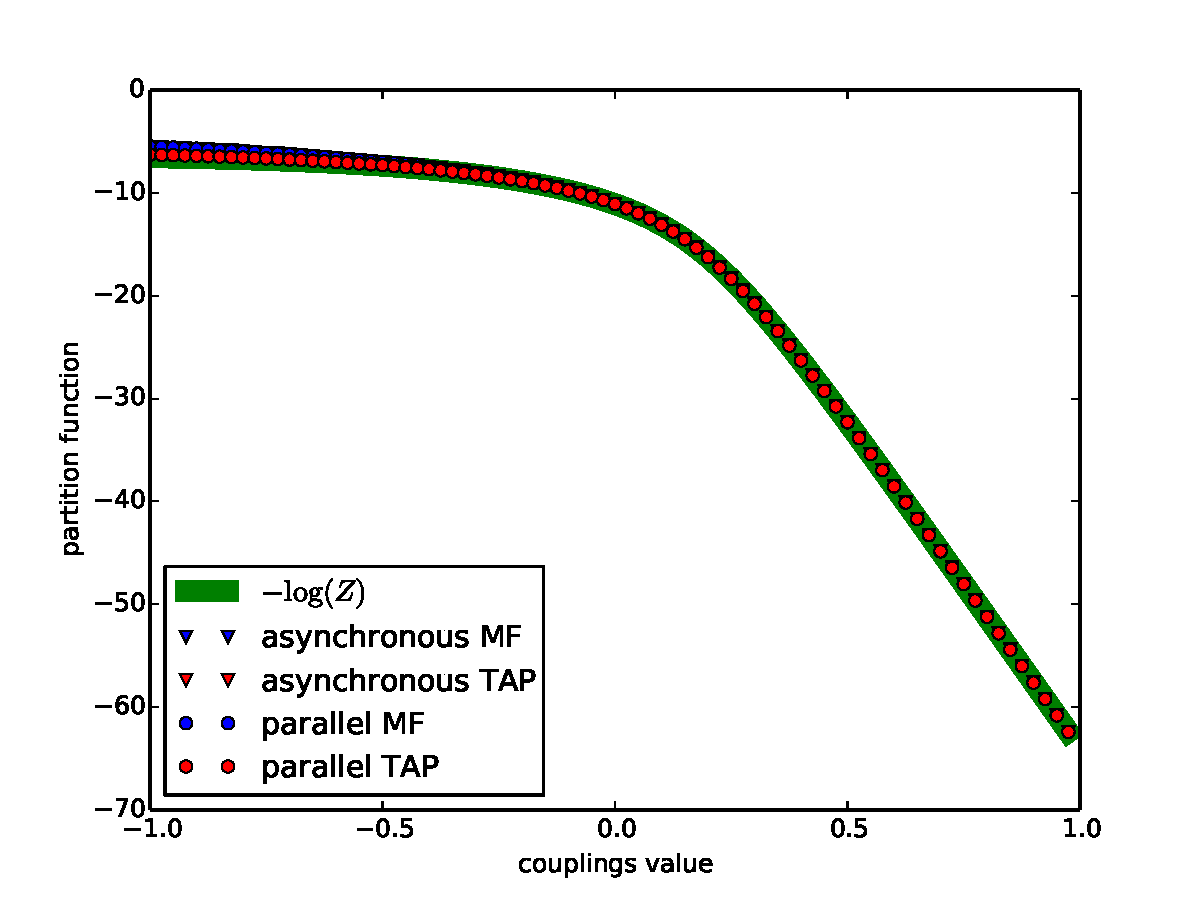
\includegraphics[width=\linewidth]{../../../Code/DRBM/toy/sameCouplingsRBMZ}
\label{fig:updates}
  \caption[1]{rbm model - same couplings}
\end{figure}
In the case of a fixed point algorithms, it is a common practice to use damped updates \cite{murphy2012machine} of the form:
$$ m_i^{t} = (1- \lambda) m_i^{t-1} + \lambda(\text{update}),$$
for $0 <\lambda<1$. This helps in avoiding unnecessary artefacts and oscillations. In all experiments conducted in this and the following chapters, the updates will be damped with $\lambda$ set to $0.5$.

\subsection{Toy models}
As it was mentioned in the previous chapter unlike naive mean field approach, the TAP approximation doesn't provide us with an upper or lower bound for the variational free energy. In our case, to specialize to the RBM model we set $\beta$ to $1$ which means that the temperature is also $1$ while the approximation was derived with infinite temperature. This suggests  Those two facts

\subsubsection{Grid toy model}
The analysis will be made assuming that the parameters of the model are known. A small grid toy model was considered of size $4 \times 4$ with periodic boundary conditions in order to avoid edge effects -- Figure \ref{fig:gridPlot} (left) shows this model from graphical models perspective. The nature of the models implies that the asynchronous updates of magnetizations seems as the most natural way to obtain a statistics of the system in the equilibrium. In this case each magnetization $m_i$ is updated one at a time using equation \ref{eq:selfConsistency}.

\begin{figure}[!htb]
\minipage{0.50\linewidth}%
% \includegraphics[width=\linewidth]{value}
\endminipage 
\minipage{0.50\linewidth}  
%\includegraphics[width=\linewidth]{policy}
\endminipage\hfill
\label{fig:gridPlot}
  \caption[1]{Grid toy model used for an exact inference.}
\end{figure}

Initially, the external field was set to $0$ and considered the case where all couplings have the same value ranging from $-1$ to $1$. As it was expected, the naive mean field approach is an upper bound for the variational free energy. However, even in the case of this small model the TAP approximation for different values of couplings is either upper or lower bound. We can see that the approximation is closest to the ground truth when the couplings are close to zero. This is consistent with the fact that the approximation was performed around point where the temperature $T$ is infinite which means that spins are independent -- small values of couplings imitate this state.

Another computational inference problem that can be evaluate thanks to the TAP method is computing a mode of the marginal density for a given spin -- in this case we can estimate average value of the spin under the Boltzmann distribution. The right plot in the Figure \ref{fig:gridModel} shows the mean squared error (MSE) between the real and estimated magnetizations for all spins. In this case, the TAP approach provides much better estimates than the naive method -- we can see that adding a second term to the approximation allows to model the connections in the system between the spins. 

\begin{figure}[!htb]
\minipage{0.50\linewidth}%
 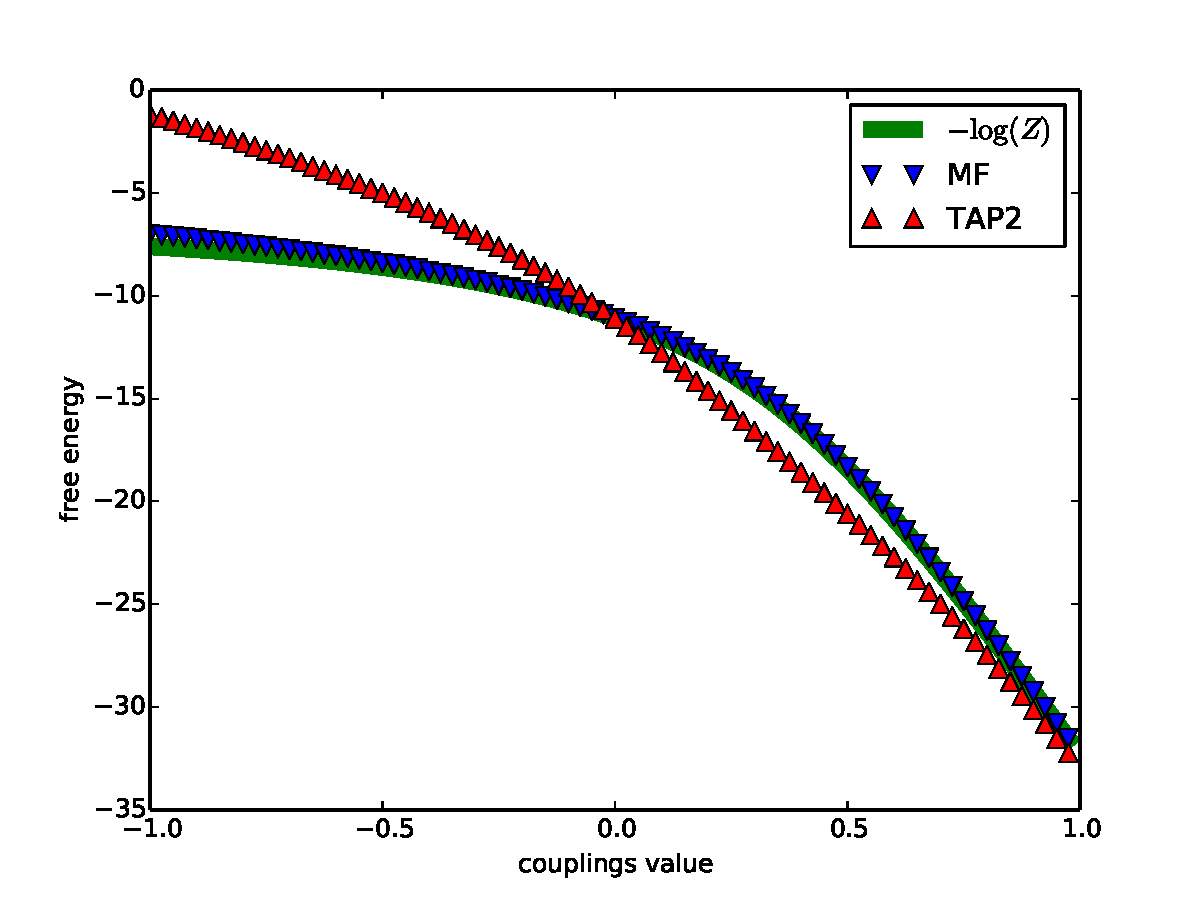
\includegraphics[width=\linewidth]{../../../Code/DRBM/toy/sameCouplingsZ}
\endminipage 
\minipage{0.50\linewidth}  
 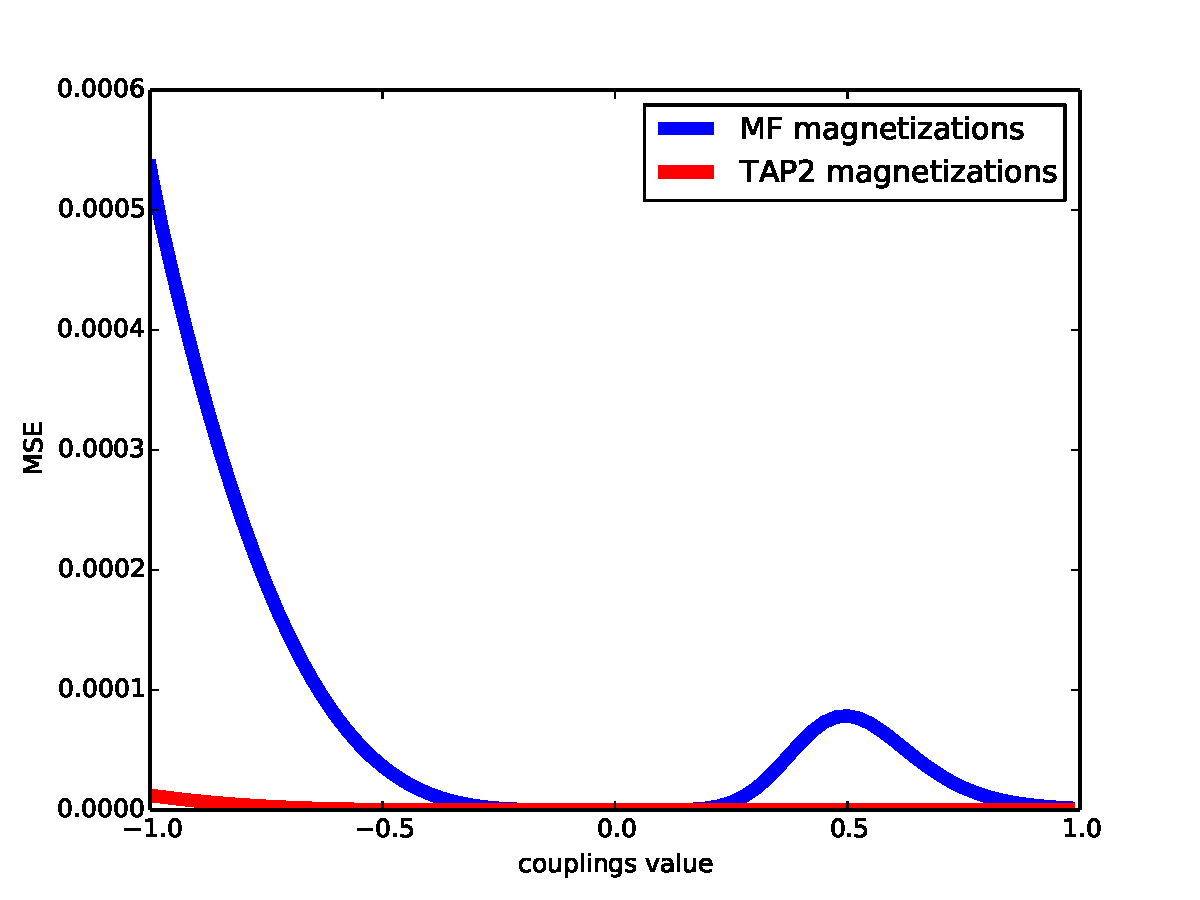
\includegraphics[width=\linewidth]{../../../Code/DRBM/toy/sameCouplingsMAG}
\endminipage\hfill
\label{fig:gridModel}
  \caption[1]{grid model - same couplings}
\end{figure}

In the next experiment, all couplings were initialised to random values around "mean" strength which varies from $0$ to $1$ and randomly assigned with $-$ sign. The results are similar to the one observed previously - Figure \ref{fig:gridModelCoup}. The naive approach gives consistently better approximation for the $-\ln Z$ while the TAP method performs better in the case of estimating average value of spin. 

\begin{figure}[!htb]
\minipage{0.50\linewidth}%
 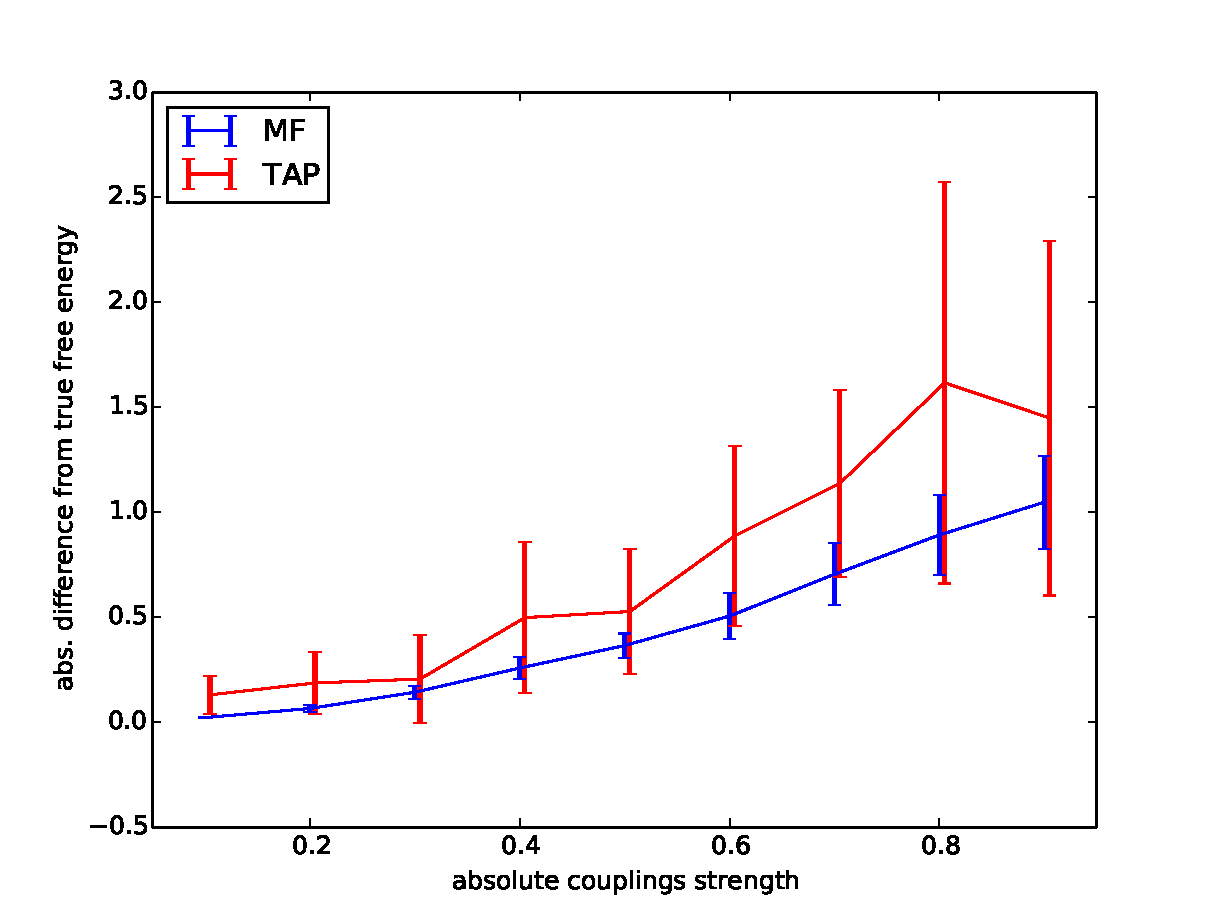
\includegraphics[width=\linewidth]{../../../Code/DRBM/toy/randomWeightsZ}
\endminipage 
\minipage{0.50\linewidth}  
 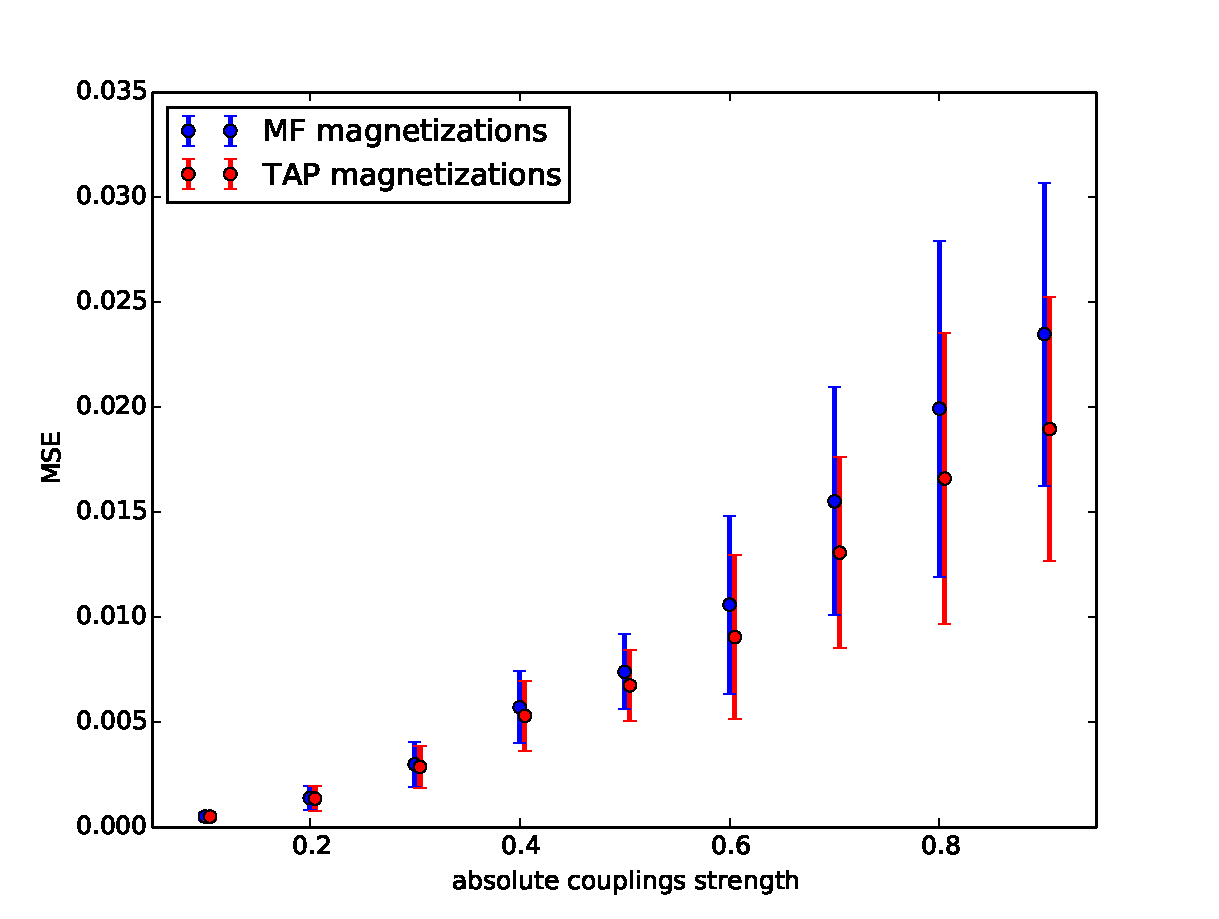
\includegraphics[width=\linewidth]{../../../Code/DRBM/toy/randomWeightsMAG}
\endminipage\hfill
\label{fig:gridModelCoup}
  \caption[1]{grid model - different couplings}
\end{figure}
TODO: add third way of noise?  -1 +1
TODO: external fields.

\subsubsection{RBM toy model}
As the -- As we will observe, due to the different structure of connections between states, 
Unlike in the previous case, there is no strong heuristics how the updates of self-consistency relations should be performed. The literature suggests that the updates in the case of the naive approach it is necessary to run self-constiency equations sequentialy \cite{welling2002new}. That is why, I considered three ways in which we can update the magnetizations. (sequential), (parallel) . The last way of performing updates follows from the application of \cite{bolthausen2014iterative} (default)
\begin{figure}[!htb]
\minipage{0.50\linewidth}%
 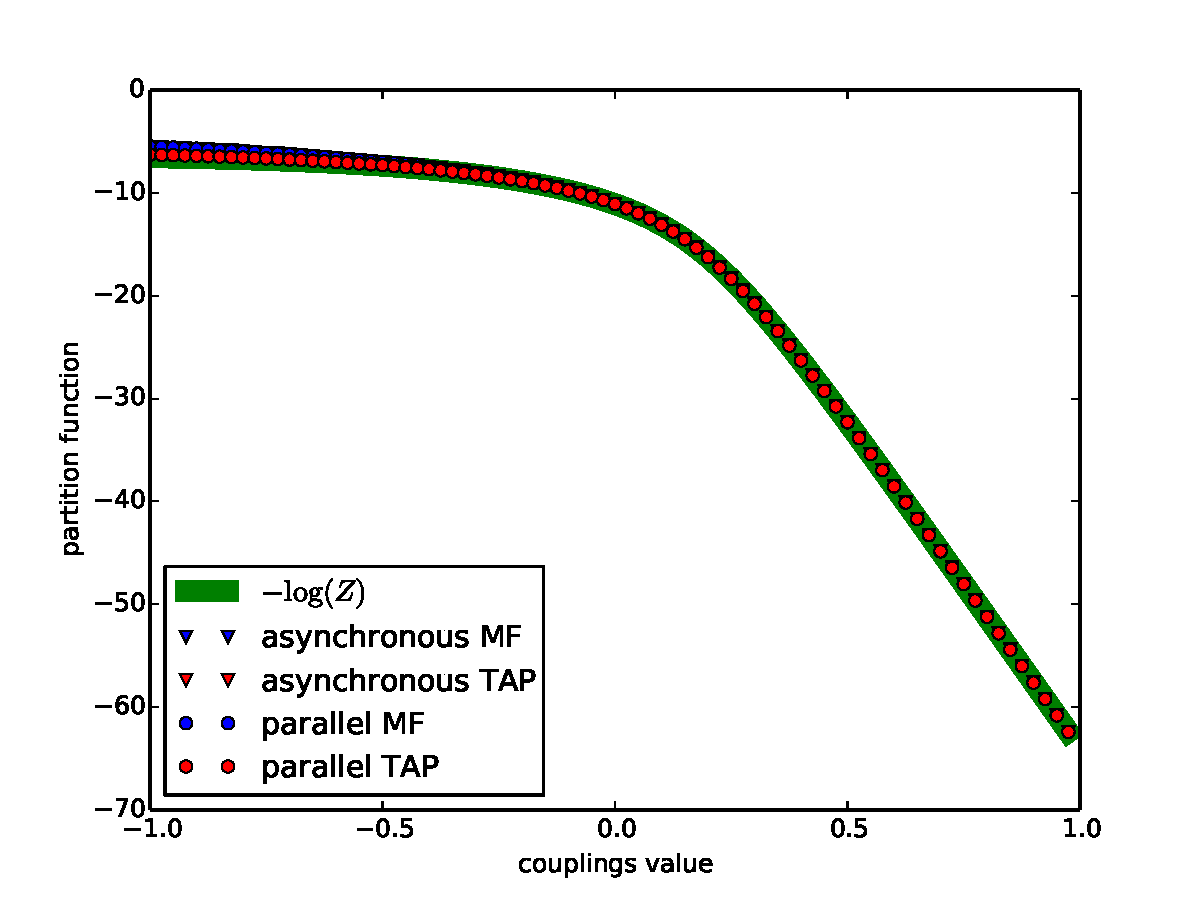
\includegraphics[width=\linewidth]{../../../Code/DRBM/toy/sameCouplingsRBMZ}
\endminipage 
\minipage{0.50\linewidth}  
 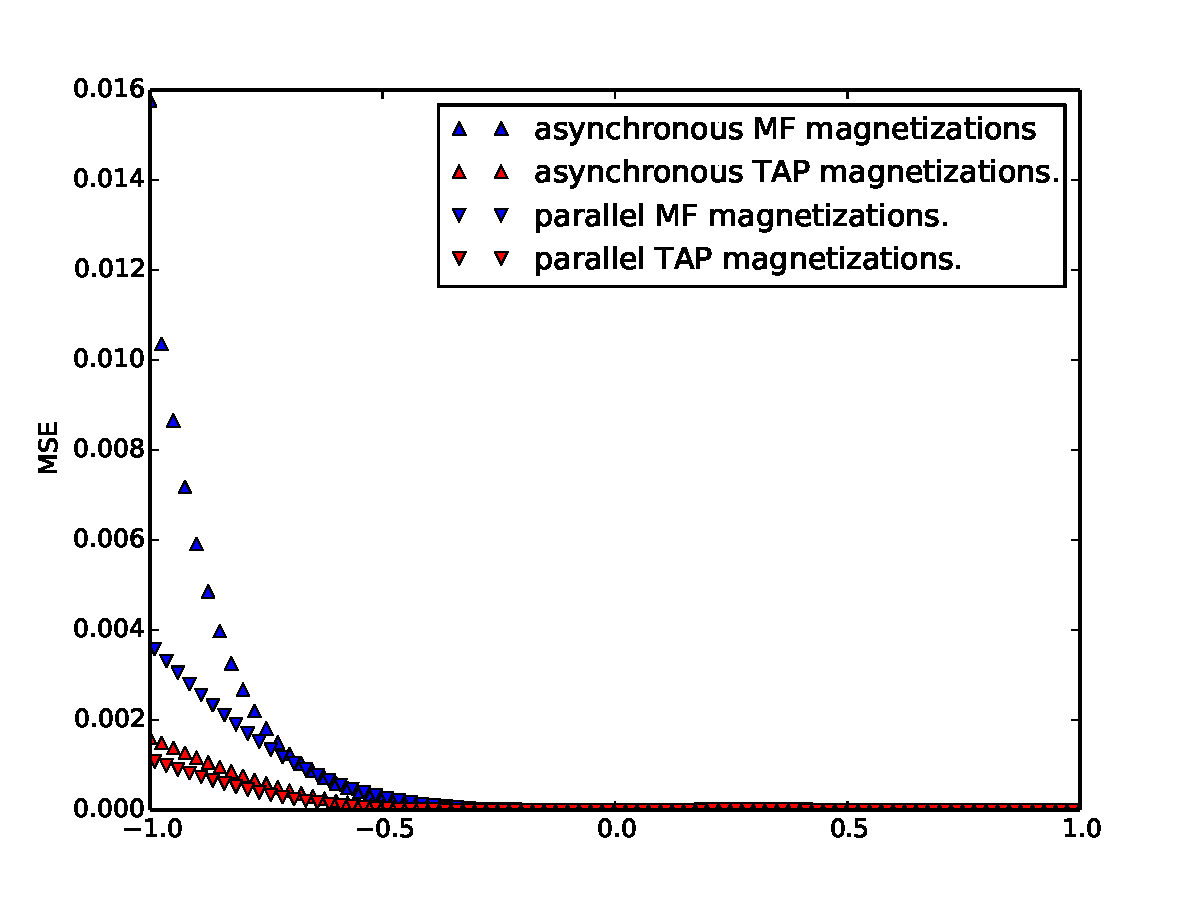
\includegraphics[width=\linewidth]{../../../Code/DRBM/toy/sameCouplingsRBMMAG}
\endminipage\hfill
\label{fig:rbmSame}
  \caption[1]{rbm model - same couplings}
\end{figure}


The results presented in Figure \ref{fig:rbmRandom} are similar to the ones obtained with.
\begin{figure}[!htb]
\minipage{0.50\linewidth}%
 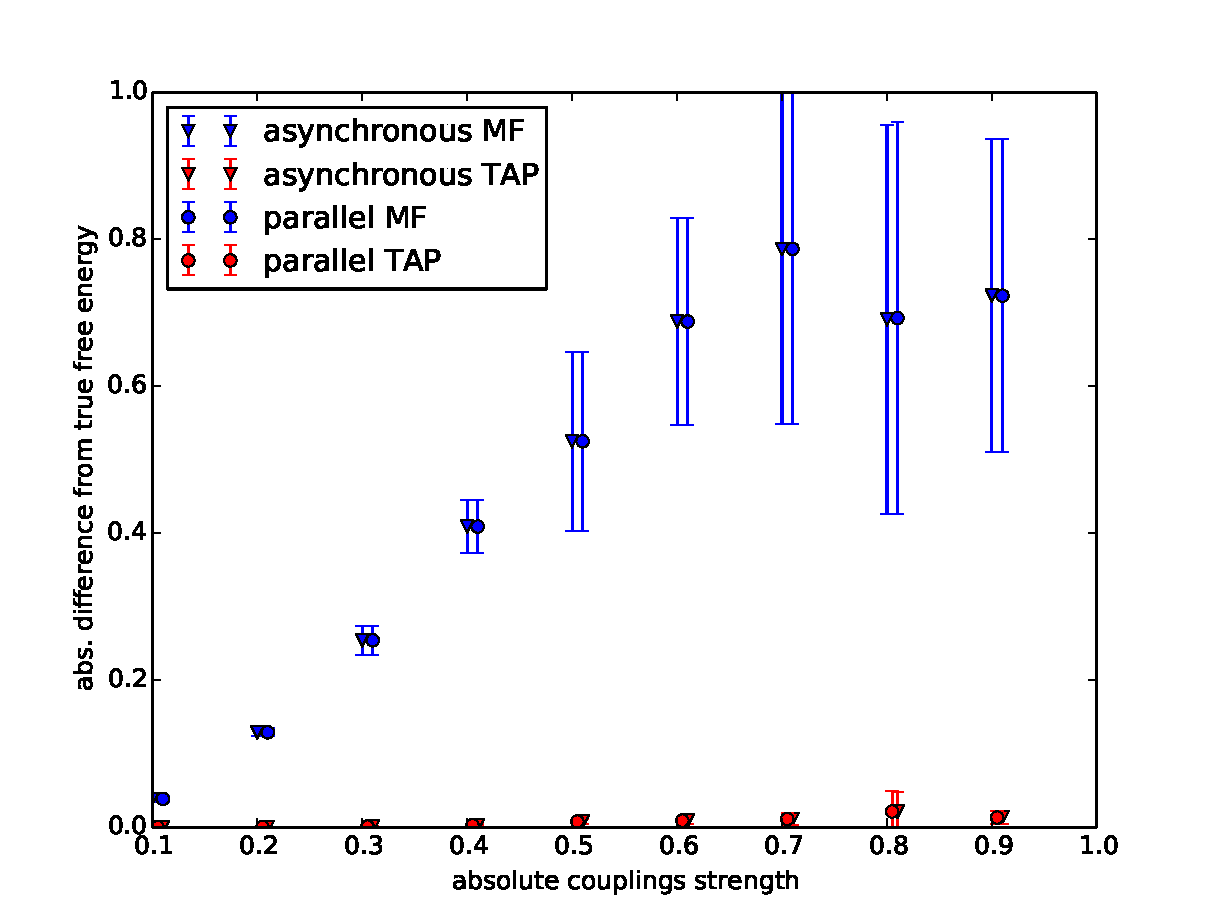
\includegraphics[width=\linewidth]{../../../Code/DRBM/toy/randomWeightsRBMZ}
\endminipage 
\minipage{0.50\linewidth}  
 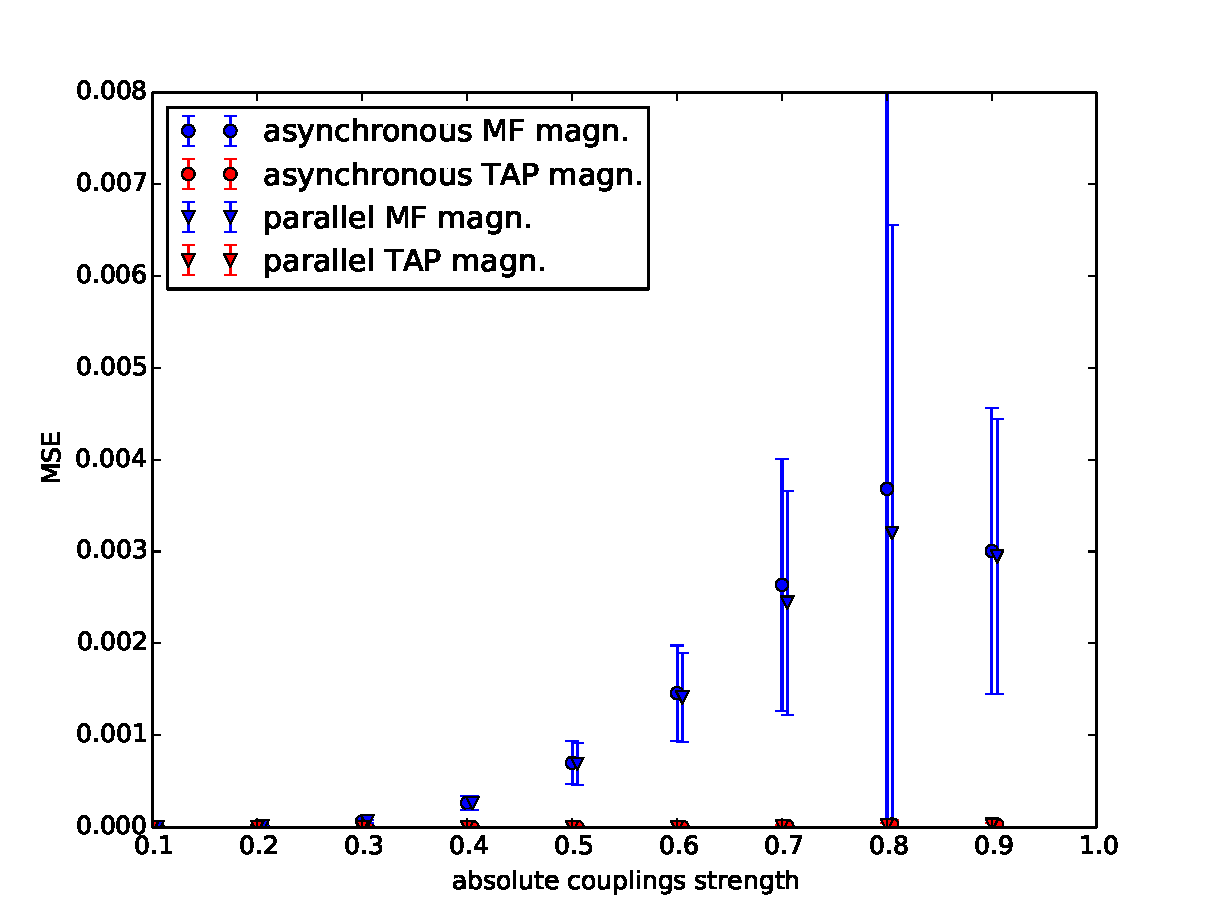
\includegraphics[width=\linewidth]{../../../Code/DRBM/toy/randomWeightsRBMMAG}
\endminipage\hfill
\label{fig:rbmRandom}
  \caption[1]{rbm model - different couplings}
\end{figure}


The results - CLT - why? TODO - might be caused 
\begin{figure}[!htb]
\minipage{0.50\linewidth}%
 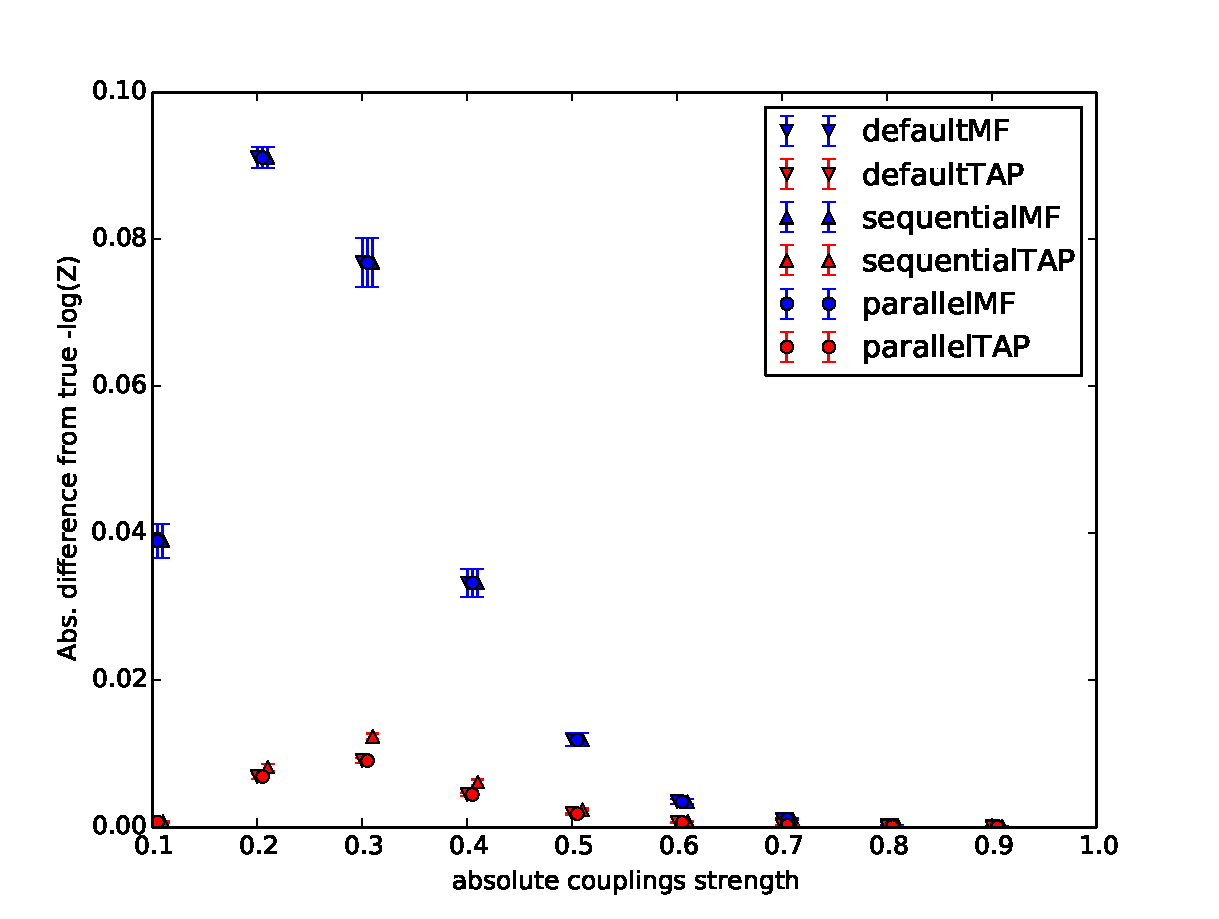
\includegraphics[width=\linewidth]{../../../Code/DRBM/toy/randomWeightsSignsRBMZ}
\endminipage 
\minipage{0.50\linewidth}  
 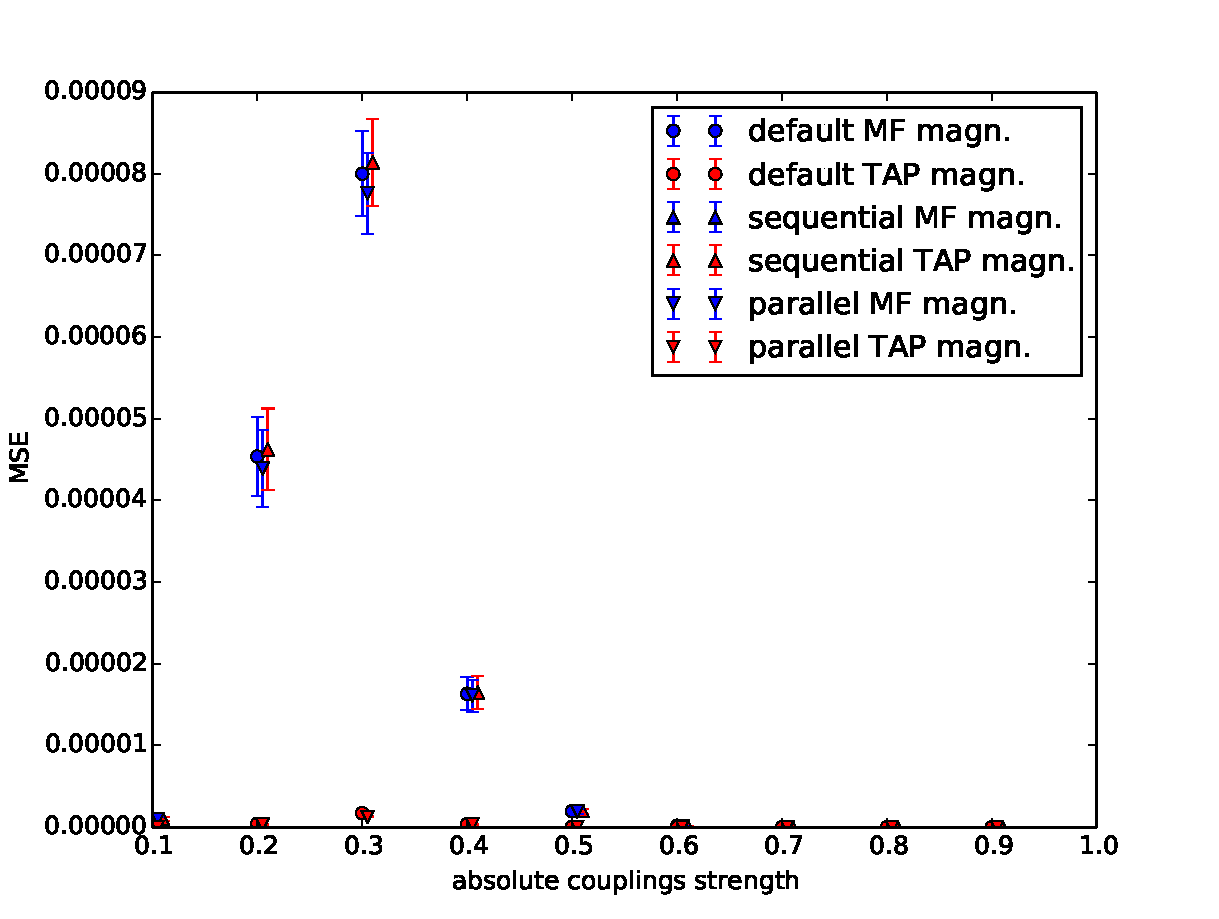
\includegraphics[width=\linewidth]{../../../Code/DRBM/toy/randomWeightsSignsRBMMAG}
\endminipage\hfill
\label{fig:gridModel}
  \caption[1]{rbm model - different signs}
\end{figure}

\newpage


\end{document}
